%!TEX root = ./slopecd.tex

\section{Theory}\label{sec:theory}
%%%%%%%%%%%%%%%%%%%%%%%%%%%%%%%%%%%%
\subsection{Directional Derivatives}%
\label{sec:directional-derivatives}
%%%%%%%%%%%%%%%%%%%%%%%%%%%%%%%%%%%%

\subsubsection{The Sorted \texorpdfstring{\(\ell_1\)}{l1}
  Norm}

\begin{theorem}
  \label{thm:sl1-directional-derivative}
  Let $v \in \bbR^p \setminus \{0\}$, \(h_0 \in \big(0, \min_{i,j \in
    \{i : \beta_i \neq 0\}}\big| |\beta_i| - |\beta_j| \big|/\max_k|v_k| \big]\) and
  define \(\sigma\) to be the permutation such that
  \[
    |\beta + h_0v|_{\sigma(1)} \geq |\beta + h_0v |_{\sigma(2)}
    \geq \cdots \geq |\beta + h_0v|_{\sigma(p)}.
  \]
  \mm{I think we need to state that for any $h \leq h_0$, $\sigma$ is still a correct reordering for $\beta + h v$ (that we use at the last line of \eqref{eq:sl1-directional-derivative})}
  The directional derivative for the sorted \(\ell_1\) norm, \(J(\beta)\), is
  \[
    D_v J(\beta) =
    \sum_{i=1}^m \sum_{j \in \mathcal{C}_i} \lambda_j v_{\sigma(j)}\sign(\beta_{\sigma(j)} + h_0v_{\sigma(j)})\]
  \mm{doesn't the definition of $h_0$ imply that $\beta_j + h_0 v_j$ has the sign of $\beta_j$?}
  \jl{Not when \(\beta = 0\), since then the sign is determined solely by \(v\).}
  where
  \[
    \mathcal{C}_i = \{j : |\beta_j| = c_i\},\qquad
    c_1 > c_2 > \cdots > c_m \geq 0,
  \]
\end{theorem}
\begin{proof}
  The directional derivative for the sorted \(\ell_1\) norm and a direction
  \(v\) with \(\lVert v \rVert = 1\) \mm{is normalization needed?}\jw{No, but I think we should put in the definition of Theorem, as it no limitation?} is
  \begin{equation}
    \label{eq:sl1-directional-derivative}
    \begin{aligned}
      D_v J(\beta) & = \lim_{h \searrow 0} \frac{J(\beta + h v) - J(\beta)}{h}                                                                    \\
                   & = \lim_{h \searrow 0} \frac{\sum_{j=1}^p\lambda_j\big(|\beta + vh|_{\sigma(j)} - |\beta|_{(j)}\big)}{h}                      \\
                   & = \lim_{h \searrow 0}\frac{\sum_i \sum_{j \in \mathcal{C}_i} \lambda_j\big(|\beta + vh|_{\sigma(j)} - |\beta|_{(j)}\big)}{h} \\
    \end{aligned}
  \end{equation}
  Assume without loss of generality that \(c_m = 0\).
  Then
  \[
    \sum_{j \in \mathcal{C}_m}\frac{\lambda_j \big( |\beta + vh|_{\sigma(j)} - |\beta|_{(j)}\big)}{h}
    = \sum_{j \in \mathcal{C}_m} \lambda_j \sign(\beta + hv)_{\sigma(j)}v_{\sigma(j)}.
  \]
  Next, recall the construction of \(h_0\) and
  observe that \(\sign(\beta_j + hv_j) = \sign(\beta_j)\)
  and \(\sigma(j) = (j)\) for all \(j \notin \mathcal{C}_m\) \mm{here there is an issue for me because, by the clustering effect, $()$ is not uniquely defined. since $v$ allows each component of $\beta + h v$ to move at different speed, we may, inside each cluster, end up with any arbitrary order (the limit on the magnitude of $h$ only imposes that vlaues from one cluster don't end up crossing another cluster )}\jw{I don't follow. You have an arbitrary ordering if $|\beta_i +hv_i|$ and $|\beta_j +hv_j|$ otherwise the ordering is defined by $\sigma$ as it determined by $\beta$ and $v$?}
  \mathurin{It's a small detail, but neither $\sigma$ nor $()$ are uniquely defined.
  For me the above sentence says that for $h$ small enough and the non zero clusters, $\sigma$ does not depend on $v$. But if you take $\beta = (0, 10, 10, 20)$ and $hv = (0, 1, 0, 0)$ or $hv = (0, 0, 1, 0)$, they don't yield the same $\sigma$.
  I'm thinking a rigorous formulation is: "$\sigma$ is a valid reordering for $\beta$"}
  whenever \(0 < h < h_0\).
  It follows that
  \[
    \sum_{j \in \mathcal{C}_i} \frac{\lambda_j\big(|\beta + hv|_{\sigma(j)} - |\beta|_{(j)}\big)}{h}
    = \sum_{j \in \mathcal{C}_i} \lambda_j\sign(\beta + vh)_{\sigma(j)}v_{\sigma(j)}.
  \]
  From this, we see that \eqref{eq:sl1-directional-derivative} reduces to
  \[
    \lim_{h \searrow 0} \sum_i \sum_{j \in \mathcal{C}_i} \lambda_j\sign(\beta + vh)_{\sigma(j)}v_{\sigma(j)}
    = \sum_i \sum_{j \in \mathcal{C}_i} \lambda_j\sign(\beta + vh_0)_{\sigma(j)}v_{\sigma(j)}.
  \]
  \mathurin{Is this reformulation equivalent? (provided $c_m = 0$)}
  \JL{Yes, but note that you still need \(h_0\) for the permutation.}
  \begin{equation*}
    D_v J(\beta) = \sum_{j \notin \cC_m} \lambda_j \sign (\beta_{\sigma(j)}) v_{\sigma(j)}
      +
    \sum_{j \in \cC_m} \lambda_j \sign (v_{\sigma(j)}) v_{\sigma(j)}
  \end{equation*}
\end{proof}

\begin{remark}
  Using \cref{thm:sl1-directional-derivative}, we see that
  the directional derivative for \eqref{eq:slope-problem} is
  \[
    D_v P(\beta) = v^T \big(\nabla L(\beta)\big) + D_v J(\beta).
  \]
\end{remark}

\subsection{Coordinate Updates}%
\label{sec:coordinate-updates}

Assume that we want to compute the coordinate update for the \(k\)th cluster
\(\mathcal{C}_k\) under the constraint that \(\sign(\beta) = s\) and
\(|\beta_j| = |\tilde \beta|\) for all \(j \in \mathcal{C}_k\).
We have
\[
  \begin{aligned}
    P(\beta) & =  \frac{1}{2} \lVert y - X\beta\rVert_2^2 + J(\beta)                                                                                                                                                                                                                                   \\
             & = \frac{1}{2} \lVert y - X_{\bar{\mathcal{C}_k}} \beta_{\bar{\mathcal{C}_k}} - \big(X_{\mathcal{C}_k} s_{\mathcal{C}_k}\big)\tilde\beta  \rVert_2^2 + \sum_{j \notin {\mathcal{C}_k}} \lambda_{(j)^-}|\beta_k| + \bigg(\sum_{j \in {\mathcal{C}_k}} \lambda_{(j)^-}\bigg)|\tilde\beta|.
  \end{aligned}
\]
Now let \(\tilde y = X_{\bar{\mathcal{C}_k}} \beta_{\bar{\mathcal{C}_k}}\)
such that \(y - \tilde y\) is the \emph{partial residual} and take the
derivate with respect to \(\tilde\beta\), yielding
\begin{equation}
  \label{eq:cluster-grad}
  \partial_{\tilde\beta}
  P(\beta) = (\tilde y - y)^T X_{\mathcal{C}_k} s_{\mathcal{C}_k} + s_{\mathcal{C}_k}^T X_{{\mathcal{C}_k}}^T X_{\mathcal{C}_k} s_{\mathcal{C}_k} \tilde\beta + \partial_{\tilde\beta}\Bigg(\bigg(\sum_{j \in {\mathcal{C}_k}} \lambda_{(j)^-}\bigg)|\tilde\beta| + \sum_{j \notin \mathcal{C}_k}\lambda_{(j)^-}|\beta_k|\Bigg),
\end{equation}
where the last term is the partial subdifferential of the sorted \(\ell_1\)
norm.
The optimality condition for this sub-problem is \(\boldsymbol{0} \in
\partial_{\tilde \beta} P(\beta).
\)

\begin{theorem}
  \label{thm:cluster-subdifferential}
  The partial subdifferential for the sorted \(\ell_1\) norm with respect
  to \(\tilde\beta\), \(\mathcal{B} \gets \mathcal{C}_k\) is
  \[
    \partial =
    \begin{cases}
      \big[-\sum_{j=|C(0)|-|\mathcal{B}|}^{|C(0)|}\lambda^{C(0)}_j, \sum_{j=|C(0)|-|\mathcal{B}|}^{|C(0)|}\lambda^{C(0)}_j\big]                            & \text{if } \tilde\beta = 0           \\
      \big[\sum_{j=|\mathcal{C}_i| - |\mathcal{B}|}^{|\mathcal{C}_i|}\lambda^{\mathcal{C}_i}_j, \sum_{j=1}^{|\mathcal{B}|}\lambda^{\mathcal{C}_i}_j\big]   & \text{if } \tilde\beta = c_i \neq 0  \\
      \big[-\sum_{j=1}^{|\mathcal{B}|}\lambda^{\mathcal{C}_i}_j, -\sum_{j=|\mathcal{C}_i| - |\mathcal{B}|}^{|\mathcal{C}_i|}\lambda^{\mathcal{C}_i}_j\big] & \text{if } \tilde\beta = -c_i \neq 0 \\
      \{\sign(\tilde\beta)\boldsymbol{1}^T\lambda^{C(\tilde\beta)}\}                                                                                       & \text{otherwise.
      }
      % \{\sign(\tilde\beta) S\big(C(\tilde\beta)\big)\}                                                                                                & \text{if } \tilde\beta \neq c_i \neq 0, \\
      % [-S(\mathcal{C}_m), S(\mathcal{C}_m)]                                                                                                           & \text{if } \tilde\beta = 0,             \\
      % [\sign(\tilde\beta)S\big( C(c_i - \sign(\tilde\beta)\varepsilon_i)\big), \sign(\tilde\beta)S\big(C(c_i + \sign(\tilde\beta)\varepsilon_i)\big)] & \text{if } |\tilde\beta| = c_i,
    \end{cases}
  \]
\end{theorem}
\begin{proof}
  Let \(f(\tilde\beta) = |\tilde\beta|\sum_{j \in \mathcal{C}_k}\lambda_{(j)^-} + \sum_{j \notin \mathcal{C}_k} \lambda_{(j)^-}|\beta_j|\).
  \(g\) is a subgradient of \(f\) at \(x\) if
  \begin{equation}
    \label{eq:subgrad-ineq}
    |y|\sum_{j \in C(y)}\lambda_{(j)^-} + \sum_{j \notin C(y)}\lambda_{(j)^-}|\beta_j|
    \geq |x|\sum_{j \in C(x)} \lambda_{(j)^-} + \sum_{j \notin C(x)}\lambda_{(j)^-}|\beta_j| + g(y - x)
  \end{equation}
  for all \(y \in \mathbb{R}\).
  Without loss of generality, since \(f\) is convex, assume that we have
  a vector \(\beta\) such that there are two clusters: one corresponding
  to \(\tilde\beta\), which we are optimizing over, and
  one additional cluster \(\mathcal{C}_q\) with corresponding
  coefficient \(c_q\).
  Then we can rewrite \eqref{eq:subgrad-ineq} as
  \[
    |y|S\big(C(y)\big) + c_q S\big(\widebar{C(y)}\big) \geq
    |x| S\big(C(x)\big) + c_q S\big(\widebar{C(x)}\big) + g(y - x).
  \]
  First observe that any \(g\) is permissible whenever \(x = y\).

  At \(x = 0\), \eqref{eq:subgrad-ineq} reduces to
  \[
    |y|S\big(C(y)\big) + c_q S\big(\widebar{C(y)}\big)
    \geq c_q(\mathcal{C}_1) + gy.
  \]
  Because \(f\) is convex, it is sufficient to consider \(|y| < c_q\),
  in which case \(C(y) = \mathcal{C}_1\) and hence
  \begin{equation}
      |y|S(\mathcal{C}_2) + c_q S(\mathcal{C}_1) \geq c_q(\mathcal{C}_1) + gy \implies
      |y|S(\mathcal{C}_2) \geq gy,
  \end{equation}
  which means that \(-S(\mathcal{C}_2) \leq g \leq S(\mathcal{C}_2)\).

  If \(x = c_q\), \eqref{eq:subgrad-ineq} becomes
  \[
    |y|S\big(C(y)\big) + x S\big(C(x)\big) \geq x(S(\mathcal{C}_1) + S(\mathcal{C}_2)) + g(y - x).
  \]
  For \(y > x\) we have \(C(y) = \mathcal{C}_1\) and consequently
  \[
    y\big(S(\mathcal{C}_1) - g\big) + x\big(g - S(\mathcal{C}_1)\big) \geq 0,
  \]
  which means that \(g \leq S(\mathcal{C}_1)\).
  Then, for \(0 < y < x\), we see
  \[
    y\big(S(\mathcal{C}_2) - g\big) + x(g - S(\mathcal{C}_2)\big) \geq 0,
  \]
  and hence \(g \geq S(\mathcal{C}_2)\).
  Using the same argument for \(x = -c_q\), we find that we in this case
  must have \(g\) such that
  \(-S(\mathcal{C}_1) \geq g \geq - S(\mathcal{C}_2)\).
  For all other choices of \(x\), \(f\) is differentiable with
  derivative \(\sign(\tilde\beta)S\big(C(\tilde\beta)\big)\).
\end{proof}

The objective and subgradient for the cluster-wise problem are shown in
\cref{fig:cluster-grad-obj}.

\begin{figure}[htbp]
  \centering
  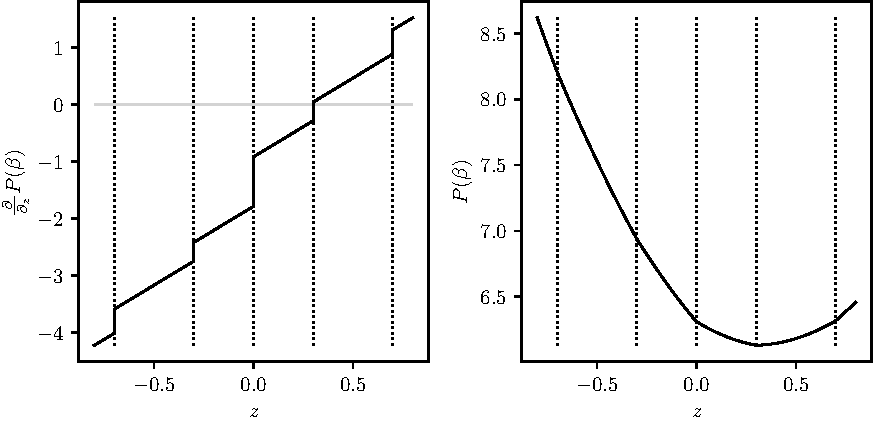
\includegraphics[]{clusterupdate-grad-obj}
  \caption{%
    Objective and gradient under the constraint that we have a fixed
    cluster.
    The optimum is found at \(\tilde\beta = 0.3\).
  }%
  \label{fig:cluster-grad-obj}
\end{figure}

Let \(\mathcal{B}\) be a cluster initialized to \(\mathcal{C}_k\), with
corresponding coefficient \(c_k\).
Then the coordinate update for \(\beta_\mathcal{B}\) is\jl{This obviously
does not work when \(s=0\). Can we just set \(s = 1\) here? It's just
the relative signs that really matter, right?}\jw{That is a really good point. Do you think we can tie to the sign of the gradient instead?. We also will not move the zero cluster this way suspect. But it should work for any formation then sign of the gradient is the way I think?}
\[
  \beta_\mathcal{B} \gets
  s_\mathcal{B} \odot
  \frac{
    T \big(
    (y - \tilde y)^T X_{\mathcal{B}} s_{\mathcal{B}}, \lambda\big)
  }{
    s_{\mathcal{B}}^T X_{\mathcal{B}}^T X_{\mathcal{B}} s_{\mathcal{B}}
  }
\]
where
\begin{equation}
  \label{eq:slope-thresholding}
  T(a; \lambda) =
  \begin{cases}
    0                                                        & \text{if } |a| \leq \sum_{i=1}^{|\mathcal{B}|}\lambda^{C(0)}_i                                                                                                                      \\
    \sign(a)c_i                                              & \text{if } \sum_{j= |\mathcal{C}_i| - |\mathcal{B}|}^{|\mathcal{C}_i|} \lambda^{\mathcal{C}_i}_j \leq |a| - c_i \leq \sum_{j=1}^{|\mathcal{B}|}\lambda^{\mathcal{C}_i}_j \\
    \sign(a)\big(|a| - \sum_{j \in C(a)}\lambda_{(j)^-}\big) & \text{otherwise.
    }
  \end{cases}
\end{equation}
To emphasize the connection between \(T\) and the soft-thresholding operator
for the lasso, we call this operator the SLOPE-thresholding operator.
In \cref{fig:slope-thresholding}, we visualize the operator.

\begin{figure}[htbp]
  \centering
  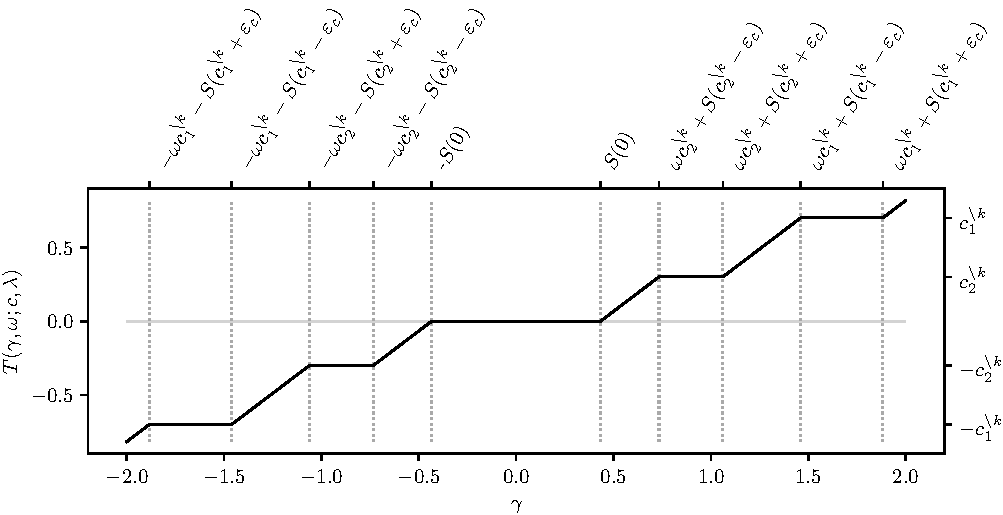
\includegraphics[]{slope-thresholding.pdf}
  \caption{The result of the SLOPE thresholding update.}
  \label{fig:slope-thresholding}
\end{figure}

\subsection{Algorithm}

Here is a rough sketch of a possible algorithm.
\begin{enumerate}
  \item Initialize \(\beta\) to zero.
  \item For each cluster,
        \begin{itemize}
          \item Check if the predictor with the largest correlation leaves the
                cluster, if not check if the two largest leave the cluster etc.
          \item If any predictors leave the cluster, compute the coordinate
                update for these predictors.
          \item If the cluster stays intact and does not correspond to the
                zero cluster, update the coefficient (common coordinate) for that
                cluster.
        \end{itemize}
\end{enumerate}
It is hopefully sufficient to only check if the coefficient with the
largest gradient splits from the cluster for most of the iterations since
checking all possible combinations of a cluster likely is expensive.
We have
to hope that's it's rare for multiple coefficients to leave a cluster in
a new cluster.
